\section{Introduction}

Collecting detailed information about wild animals~\cite{Prangle2006NewRadiocolars,Rutz2012AutomatedMapping} 
remains a significant technical challenge that
limits the ability of Ecologists to study them, the interactions between them, and the interactions 
between wild animals and their environment. One tools that has emerged a little over a decade ago
and has been gaining significance is 
{\em encounter detection and logging}~\cite{Tentelier2016FishNetwork,
Bohm2009WildlifeLivestock,Ripperger2016ProximitySensing}.

Encounter detection systems~\cite{Levin2015Performance,Menhill2012NovelTelemetry,dressler2016bats} 
consist of radio devices called {\em tags} that are attached to wild
animals (and sometimes also to fixed positions and to livestock), as depicted in Fig.~\ref{tags}. 
The radios transmit identification
packets periodically, usually once every few seconds. The radios also listen to such packets, not
necessarily continuously, and record data about received packets in persistent memory on the tag. The
radios are typically configured for short-range communication by using low transmit power and by 
using high data-rates (both limit the signal-to-noise ratio at the receiver). Because the radios
are configured for short-range communication, receiving a packet implies that the transmitting tag is
in close proximity to the receiving tag. Recent systems record with each packet a received signal strentgh
indication (RSSI)~\cite{Daiya2011Experimental}, which helps to estimate the distance between the transmitter and receiver.
This is the main goal of these systems: to log close-proximity
events between two or more animals. The logs are downloaded either by physically retrieving the tags,
or remote download to base-stations placed in locations that the animals are known to frequent.

Such systems have gained popularity among Ecologists because the tags are relatively inexpensive and can
be very small, because deployment does not require much infrastructure in the field, and because close-proximity
encounters are key aspects of many significant events in the life of animals: mating, predation, transmission of infectious
diseases, and so on. We comment on some of these applications in Section~\ref{sec:related-work}.

\begin{figure}[!t]
    \centering
    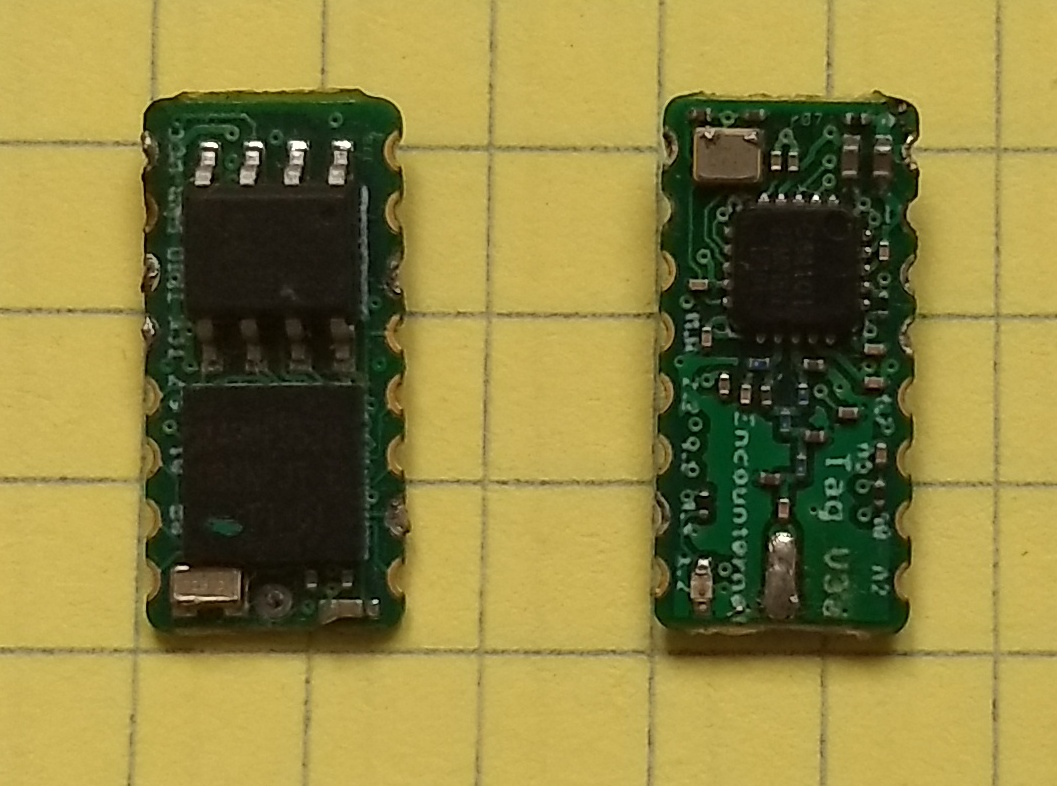
\includegraphics[width=3in]{figures/tag}
    \caption{Tags attached to wild animals. Tags use a tiny printed-circuit board 
    and could be powered by miniature batteries.
    The small batteries restrict the life-span of tags and increase the importance of effective protocols.}
    \label{tags}
\end{figure}

Encounter-registration systems pose challenging protocol-ralated problems. One problem is to minimize
the power used for listening to other tags. All of the systems developed so far have used low-power integrated
UHF transceivers, and the power consumed by these while receiving is comparable to the power that they use
to transmit. The dominant strategy to address this issue appears to be duty-cycling the 
receiver~\cite{Zhang2017Performance}, so that it is
off most of the time. Synchronizing the timing of the activity periods of all tags can minimize total receive energy
while maximizing that transmissions will be received. If tags do not synchronize their activity periods, many transmissions
at close proximity may go unnoticed; this is not an unreasonable solution if encounters are long. Another emerging approach
to the receive-power problem is based on so-called {\em wake-up receivers}, specialized nano-power sub-receivers whose only
job is to wake up the main receiver when a strong packet is received. These have not been used in Ecology research so we
exclude them from most of the discussion; we do comment on them in Section~\ref{sec:related-work}.

The other protocol-related problem is interference. 
If many tags transmit simultaneously, receiving tags may fail
to reconstruct valid packets. Paradoxically, highly-efficient 
systems with good time synchronization and short activity
periods suffer more from this problem than less efficient systems 
in which the clocks of tags are not synchronized tightly
enough to transmit simultaneously. This is not a theoretical problem; 
many species of animals, including many species of
birds and bats, roost together, so encounters of tens or hundreds 
of individuals are not necessarily rare.

Our fundamental observation is that it is a waste of 
energy if an animal is not encountering with others
while still keeps the tag working frequently.
Thus it is reasonable for a tag to
increase the working frequency of its radio when 
encounter happens; otherwise it keeps
the radio in a low-power mode. The key is to design a mechanism
to identify the existence of an encounter in real-time. 



In this paper, we propose an effective protocol for encounter registration, 
addressing these two problems systematically and
methodically. In our protocol, we design two stages for the tags, 
namely detecting stage and connecting stage.
In the detecting stage, a tag works a fraction of time in order to save energy,
and transmits a beacon periodically to detect whether an encounter is happening at the moment.
When detected an acknowledgement, the tag switches to the connecting stage and increases the 
transmission frequency in order to establish links with other tags. To deal with interference 
caused by 
In the connecting stage,
a tag adaptively adjusts its transmission probability: it increases the probability when 
the channel is detected idle and reduces the probability when interference is detected.  


We present concrete analysis of the protocol under our radio model
and carry out a number of experiments to validate this model.
We prove that our protocol accomplishes the encounter registration
of $k$ tags in $O(k)$ slots time.


%% Remaining structure
The remainder of the paper is organized as follows. 
The next section highlights the related works.
Section~\ref{sectionmodel} presents the system model and basic definitions.
We present the concrete protocol design
in Section~\ref{sectionprotocol}. We  
analyze the performance of our protocol in Section~\ref{sectionanalysis}. 
We validate the radio model by real experiments in Section~\ref{sectionsimulation}, 
and the paper is concluded in Section~\ref{sectionconclusion}.